   
        
        \begin{ledgroupsized}[r]{120mm}
        \footnotesize 
        \pstart        
        \noindent\textbf{\"{U}berlieferung:}  
        \pend
        \end{ledgroupsized}
      
       
              \begin{ledgroupsized}[r]{114mm}
              \footnotesize 
              \pstart \parindent -6mm
              \makebox[6mm][l]{\textit{L}}Konzept: LH XXXVII 2 Bl. 101. 1 Bl. 2\textsuperscript{o}. 1 S. In der oberen H\"{a}lfte links zwei Zeichnungen und eine Marginalie. Text umlaufend. Bei der ersten Zeichnung handelt es sich um einen verworfenen Ansatz zu \textit{[Fig. 1]}, der aufgrund fehlender Signifikanz im Druck keine Ber\"{u}cksichtigung findet. Geringe Textverluste durch Papierabbruch am unteren Rand. R\"{u}ckseite leer.\pend
              \end{ledgroupsized}
       
              \begin{ledgroupsized}[r]{114mm}
              \footnotesize 
              \pstart \parindent -6mm
              \makebox[6mm][l]{\textit{E}}\cite{00243}\textsc{Gerland} 1906, S.~53f.\\Cc 2, Nr. 493 \pend
              \end{ledgroupsized}
        %\normalsize
        \vspace*{5mm}
        \begin{ledgroup}
        \footnotesize 
        \pstart
      \noindent\footnotesize{\textbf{Datierungsgr\"{u}nde}: Leibniz hat sich offenbar erst in Paris ausf\"{u}hrlicher mit der Cartesischen \cite{00038}\textit{Optik} auseinandergesetzt. Textzeugen dieser Rezeption sind die \textit{Demonstratio nova legum refractionis quae in lumine observantur}, \cite{00265}N. 21, sowie der kurze Auszug aus der \cite{00038}\textit{Dioptrice} des Descartes, N. 20. In dem vorliegenden Text f\"{u}hrt er die in N. 21 begonnene Auseinandersetzung mit Descartes'\protect\index{Namensregister}{\textso{Descartes} (Cartesius, des Cartes, Cartes.), Ren\'{e} 1596\textendash 1650} Brechungsgesetz anhand des \cite{00087}\textit{Trait\'{e} de physique} von Rohault fort. Wir gehen f\"{u}r diese Texte von einem gemeinsamen Entstehungszeitraum aus, den wir N. 21 folgend festsetzen. Die Datierung wird durch das Wasserzeichen gest\"{u}tzt, das dem auf LH XXXVII 2 Bl. 97 entspricht.}
        \pend
        \end{ledgroup}
      
        \vspace*{8mm}
        \pstart 
        \normalsize
      [101 r\textsuperscript{o}] In Cartesii\protect\index{Namensregister}{\textso{Descartes} (Cartesius, des Cartes, Cartes.), Ren\'{e} 1596\textendash 1650} doctrina de refractione\protect\index{Sachverzeichnis}{refractio} multiplex error inest. Supponit ipse et ex eo Rohaultius\protect\index{Namensregister}{\textso{Rohault} (Rohaultius), Jacques 1620\textendash 1675} \edtext{p. 1. c. 15. 11.}{\lemma{}\Afootnote{p. 1. c. 15. 11. \textit{ erg.} \textit{ L}}}\edtext{}{\lemma{11.}\Bfootnote{\textsc{J. Rohault, }\cite{00087}\textit{Trait\'{e} de physique}, Teil 1, Paris 1671, S.~116f.}} novum medium densius obstare solum perpendiculariter, non vero horizontaliter, quod falsum est, nisi in momento primo, secus in sequentibus. Hinc et \edtext{recte}{\lemma{et}\Afootnote{ \textit{ (1) }\ male \textit{ (2) }\ recte \textit{ L}}} ait pilam perdere dimidium suae celeritatis\protect\index{Sachverzeichnis}{celeritas} si in medium \edtext{duplo}{\lemma{}\Afootnote{duplo \textit{ erg.} \textit{ L}}} densius ingrediatur, sed hoc non potest conciliare cum priore Hypothesi, ubi horizontali conatui nihil ademit. Cogitur ergo \edtext{supponere corpus}{\lemma{supponere}\Afootnote{ \textit{ (1) }\ interesse \textit{ (2) }\ corpus \textit{ L}}} reflecti non refringi, si angulus incidentiae\protect\index{Sachverzeichnis}{angulus!incidentiae} sit minor 45 graduum. Imo inesse videtur error delineationi et calculo Rohaultii\protect\index{Namensregister}{\textso{Rohault} (Rohaultius), Jacques 1620\textendash 1675} dict. prop. XI.\edtext{}{\lemma{XI.}\Bfootnote{\textsc{J. Rohault}, \cite{00087}a.a.O., S.~116.}} Ponamus enim lineam \textit{ab} describi intervallo unius minuti lineam \textit{bm} intervallo 2 minutorum, ob dimidiatam celeritatem\protect\index{Sachverzeichnis}{celeritas} in medio duplo resistentiore. Ponamus \edtext{cum Rohaultio\protect\index{Namensregister}{\textso{Rohault} (Rohaultius), Jacques 1620\textendash 1675}}{\lemma{}\Afootnote{cum Rohaultio\protect\index{Namensregister}{\textso{Rohault} (Rohaultius), Jacques 1620\textendash 1675} \textit{ erg.} \textit{ L}}} et celeritatem\protect\index{Sachverzeichnis}{celeritas} non nisi conatus \edtext{perpendicularis \textit{pb}}{\lemma{conatus}\Afootnote{ \textit{ (1) }\ horizontalis in \textit{ph} \textit{ (2) }\ perpendicularis \textit{pb} \textit{ L}}} aut \textit{bh} \edtext{dimidiari}{\lemma{\textit{bh}}\Afootnote{ \textit{ (1) }\ minui \textit{ (2) }\ dimidiari \textit{ L}}}, celeritatem in \textit{bd} horizontali manere. Ergo in duobus minutis describet lineam \textit{bl} \edtext{vel \textit{om}}{\lemma{}\Afootnote{vel \textit{om} \textit{ erg.} \textit{ L}}} duplam lineae prioris horizontalis descriptae \textit{ag} vel \textit{fb}. Hactenus recte Rohaultius\protect\index{Namensregister}{\textso{Rohault} (Rohaultius), Jacques 1620\textendash 1675}.
         \begin{wrapfigure}{l}{0.5\textwidth}          
         \includegraphics[width=0.5\textwidth]
%  Zeitz       {images/37_2_101r1}
 {images/LH37_2_101r-fig1}
         \\\centering\textit{[Fig. 1]}
         \end{wrapfigure}
      Sed \edtext{in iisdem duobus minutis non debet percurrere}{\lemma{Sed}\Afootnote{ \textit{ (1) }\ per consequens in \textit{ (2) }\ in [...] percurrere \textit{ L}}} dimidiam \edtext{perpendicularis}{\lemma{dimidiam}\Afootnote{ \textit{ (1) }\ horizontalis \textit{ (2) }\ perpendicularis \textit{ L}}} \textit{gb} nempe \textit{bo} ut vult Rohaultius\protect\index{Namensregister}{\textso{Rohault} (Rohaultius), Jacques 1620\textendash 1675}, ita enim celeritas\protect\index{Sachverzeichnis}{celeritas} erit quadruplo minor, si enim duobus minutis dimidium describit ejus quod alias uno. Sed debet duobus minutis describere lineam \textit{bh}, \textit{m} ergo extra circulum cadet. Quare necesse est \edtext{locum pilae}{\lemma{}\Afootnote{locum pilae \textit{ erg.} \textit{ L}}} cadere extra circulum in \textit{q} contra Hypothesin. Imo impossibile est supposita dimidiatione celeritatis\protect\index{Sachverzeichnis}{celeritas} lineae explicare compositiones. Retineantur enim duobus minutis eaedem lineae, manifestum est \edtext{corpus perventurum}{\lemma{corpus}\Afootnote{ \textit{ (1) }\ recta \textit{ (2) }\ perventurum \textit{ L}}} esse duobus minutis eodem quo antea uno sine ulla refractione\protect\index{Sachverzeichnis}{refractio}, ac proinde in sola celeritate\protect\index{Sachverzeichnis}{celeritas} non in determinatione fiet mutatio. Quaerendum est unde veniat resistentia corporis an ab Elatere\protect\index{Sachverzeichnis}{elater}. Si corpus pure Elasticum est, restituet se in statum priorem. \edtext{Sed nullum corpus perfecte se restituit, verum aliud alio magis, uti videmus}{\lemma{Sed}\Afootnote{ \textit{ (1) }\ quia nullum corpus perfecte se restituit, aliudque alio magis, hinc nullum corpus \textit{ (2) }\ nullum [...] videmus \textit{ L}}} altius repercuti pilam a marmore quam a ligno. Ita similiter si resistentia corporum oritur ab eorum Elaterio\protect\index{Sachverzeichnis}{elater} nulla erit refractio\protect\index{Sachverzeichnis}{refractio}, sed imminutio  \edtext{celeritatis.}{\lemma{celeritatis.}\Afootnote{ \textit{ (1) }\ Sed si \textit{ (2) }\ Quia \textit{ L}}} \edtext{Quia Reactio}{\lemma{Quia}\Afootnote{ \textit{ (1) }\ Elaterium\protect\index{Sachverzeichnis}{elater|textit} \textit{ (2) }\ Reactio \textit{ L}}} est incidentiae proportionalis, ac proinde utrique conatui tam horizontali quam perpendiculari idem detrahitur in proportione non arithmetica sed geometrica. Contra si resistentia oritur non ab  Elaterio\protect\index{Sachverzeichnis}{elater}, sed a causa quadam ab incidentia non determinata, sed quae forti et debili incidentiae tantundem detrahit, ut est densitas, tenacitas, \edtext{gravitas,}{\lemma{}\Afootnote{gravitas, \textit{ erg.} \textit{ L}}} tunc et celeritas\protect\index{Sachverzeichnis}{celeritas} et determinatio minuitur, ut alibi \edtext{demonstravi.}{\lemma{demonstravi.}\Bfootnote{\textsc{G. W. Leibniz}, \cite{00256}\textit{Hypothesis physica nova}, Mainz 1671, § 22 (\cite{00256}\textit{LSB} VI, 2, S. 228\textendash 231).}} Nisi celeritas\protect\index{Sachverzeichnis}{celeritas} imminui possit, ut si sit momentanea in lumine videlicet. Ibi enim supponendum est quasi esset pila mota retenta eadem celeritate\protect\index{Sachverzeichnis}{celeritas}, quae minuto veniat ex centro in circumferentiam, sed quae ob resistentiam mutet determinationem. \pend \pstart Rohault\protect\index{Namensregister}{\textso{Rohault} (Rohaultius), Jacques 1620\textendash 1675} p. 1. c. 27. n. 38.\edtext{}{\lemma{n. 38.}\Bfootnote{\textsc{J. Rohault}, \cite{00087}a.a.O., S.~282.}} les passages de la lumiere sont deja tout faits. Hinc facilius, ire per corpora dura, quia in iis canales expolitiores. An sic dicendum est: \pend \pstart Corpus excipiens radios reagit, cedit ergo primo radio sed minus quam aliud corpus, ergo et a secundo impellitur, et a tertio, quarto, quinto, aliisque insequentibus, tanto majore celeritate\protect\index{Sachverzeichnis}{celeritas}, quanta est corporis luminaris pressio.\footnote{\textit{Unterhalb der [Fig. 1]:} Nota pressio luminis pertingit in momento per spatium quantumcunque est tum definitae celeritatis\protect\index{Sachverzeichnis}{celeritas}. } Etsi conatus sint infiniti intra datum \edtext{temporis spatium}{\lemma{datum}\Afootnote{ \textit{ (1) }\ momentum \textit{ (2) }\ temporis spatium \textit{ L}}}. Et quia in omni corpore est reactio quaedam, hinc in omni corpore reflexio\protect\index{Sachverzeichnis}{reflexio} quaedam, est et in omni corpore refractio\protect\index{Sachverzeichnis}{refractio} sed perturbata. Et quia radii lucis repetuntur saepe intra tempus minimum sensibile in unum corpus, hinc luminis sensibilitas, alioqui enim rei momentaneae sensibilitas nulla. Illuminare nihil aliud quam calefacere, id est dividere in minutas partes, motus separatos habentes. Sed hoc faciunt non singuli radii sed diversi collecti\edtext{, dum}{\lemma{collecti}\Afootnote{ \textit{ (1) }\ . Ita ut \textit{ (2) }\ , dum \textit{ L}}} unus huc, alius illuc nititur. \pend \pstart Porro quia major vis ingruit in magis reagens, hinc in magis reagente radius fortius ingruit. Hinc major vis pressionis sed quomodo hinc determinatio ad perpendicularem. An quod omne pressum reagit in perpendiculari; et quod pressio a lumine non fit nisi in perpendiculari? Imo pressio etsi obliqua sit, potest tamen dici restitutionem esse in perpendiculari. Hinc sequitur incrementum non esse nisi in perpendiculari, quia et reactio non nisi in perpendiculari.\pend \pstart Propositiones: Si corpus incidit in corpus \edtext{excipiens immobile et utrumque durum nec tamen Elasticum est,}{\lemma{corpus}\Afootnote{ \textit{ (1) }\ quod Elasticum non est nec penetrat, nec alterum ab altero penetratur et corpus excipiens immobile est, \textit{(a)}\ nec molle nec Elasticum est \textit{(b)}\ et utrumque \textit{ (2) }\ excipiens [...] est, \textit{ L}}} incidens continuat motum horizontalem omisso perpendiculari. \edtext{(Omne corpus Elasticum se restituit linea brevissima seu perpendiculari.)}{\lemma{perpendiculari.}\Afootnote{ \textit{ (1) }\ Si corpus incidens aut excipiens molle est, transfiguratur, et si tenax est, fit \textit{ (2) }\ (Omne [...] perpendiculari.) \textit{ L}}} Anguli incidentiae\protect\index{Sachverzeichnis}{angulus!incidentiae} et reflexionis\protect\index{Sachverzeichnis}{angulus!reflexionis} sunt aequales, si tanta est vis restitutionis, quanta pressionis. Si incidentia est perpendicularis etiam reflexio\protect\index{Sachverzeichnis}{reflexio} est perpendicularis etsi vis restitutionis et pressionis 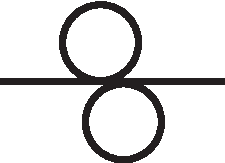
\includegraphics[width=0.05\textwidth]{images/LH37_2_101r_draw2} sint inaequales. Si incidentia et reflexio\protect\index{Sachverzeichnis}{reflexio} sunt inaequales, et incidentia fortior est, reflexio\protect\index{Sachverzeichnis}{reflexio} declinabit ad perpendicularem. Si reflexio\protect\index{Sachverzeichnis}{reflexio} fortior est incidentia declinabit a \edlabel{perpendicularistart}\edtext{perpendiculari.}{{\xxref{perpendicularistart}{perpendiculariend}}\lemma{perpendiculari.}\Afootnote{ \textit{ (1) }\ Si corpus excipiens penetratur ab \textit{(a)}\ incipiente, \textit{(b)}\ incedente, \textit{ (2) }\ Si Medium (seu corpus excipiens quod penetratur ab incidente)  \textbar\ novum \textit{ erg.}\ \textbar\ \textit{(a)}\ densius est \textit{(b)}\ magis resistit priore \textit{ (3) }\ Si [...] resistente \textit{ L}}} \pend \pstart Si corpus movetur in medio resistente\edlabel{perpendiculariend} ejus celeritas\protect\index{Sachverzeichnis}{celeritas} continue decrescit, determinatione salva. Si corpus \edtext{transit ex medio minus resistente in magis resistens}{\lemma{corpus}\Afootnote{ \textit{ (1) }\ motum ex medio magi \textit{ (2) }\ transit ex medio \textit{(a)}\ magis resistente in minus \textit{(b)}\ minus resistente in magis resistens \textit{ L}}} et \edtext{resistentia}{\lemma{et}\Afootnote{ \textit{ (1) }\ incidentia \textit{ (2) }\ resistentia \textit{ L}}} arithmetice eadem est \edtext{seu determinata}{\lemma{}\Afootnote{seu determinata \textit{ erg.} \textit{ L}}} contra incidentiam quam\-cunque primo momento \edtext{seu sub initium immersionis}{\lemma{momento}\Afootnote{ \textit{ (1) }\ refractionis\protect\index{Sachverzeichnis}{refractio|textit} \textit{ (2) }\ seu sub initium immersionis \textit{ L}}} directio \edtext{refractionis\protect\index{Sachverzeichnis}{refractio}}{\lemma{}\Afootnote{refractionis\protect\index{Sachverzeichnis}{refractio} \textit{ erg.} \textit{ L}}} est a perpendiculari. \edtext{Si nisus incidentis est continue reparatus, refractio\protect\index{Sachverzeichnis}{refractio} $\langle$in$\rangle$ medium $\langle$densius$\rangle$ Elasticum est ad perpendicularem: in medium minus Elasticum a perpendiculari.}{\lemma{}\Afootnote{Si [...] medium $\langle$densius$\rangle$  \textbar\ Elasticum \textit{ erg.}\ \textbar\ est [...] perpendiculari. \textit{ erg.} \textit{ L}}} Si vero a magis resistente transeat in minus resistens non ideo augetur celeritas\protect\index{Sachverzeichnis}{celeritas} \edtext{aut determinatio}{\lemma{}\Afootnote{aut determinatio \textit{ erg.} \textit{ L}}} (etsi \edtext{minuatur}{\lemma{(etsi}\Afootnote{ \textit{ (1) }\ augeatur \textit{ (2) }\ minuatur \textit{ L}}} resistentia seu celeritatis\protect\index{Sachverzeichnis}{celeritas} decrementum) nisi accedat nova causa. Sequentibus momentis immersionis continue minuitur directio refractionis\protect\index{Sachverzeichnis}{refractio} a perpendiculari. Si primum et ultimum momentum immersionis sint idem, seu si corpus incidens supponatur esse punctum \edtext{(et resistentia}{\lemma{(et}\Afootnote{ \textit{ (1) }\ incidentia \textit{ (2) }\ resistentia \textit{ L}}} arithmetice eadem seu determinata est), tunc si angulus incidentiae\protect\index{Sachverzeichnis}{angulus!incidentiae} est \edtext{minor}{\lemma{est}\Afootnote{ \textit{ (1) }\ major \textit{ (2) }\ minor \textit{ L}}} 45 \edtext{graduum directio reflexionis}{\lemma{graduum}\Afootnote{ \textit{ (1) }\ reflexio\protect\index{Sachverzeichnis}{reflexio|textit} \textit{ (2) }\ directio reflexionis \textit{ L}}} erit a perpendiculari, si major ad perpendicularem. (Aliud est directio reflexionis\protect\index{Sachverzeichnis}{reflexio} aut refractionis\protect\index{Sachverzeichnis}{refractio} aliud reflexio\protect\index{Sachverzeichnis}{reflexio} aut refractio\protect\index{Sachverzeichnis}{refractio} ipsa. Directio conatus, ipsa reflexio\protect\index{Sachverzeichnis}{reflexio} etc., motus, uti directionem habet a tangente quod movetur circa centrum). Idem est si pressio transeat de medio in medium. Si resistentia \hspace{1mm}medii est \hspace{1mm}geometrice eadem, seu \hspace{1mm}proportionalis incidenti, refractio\protect\index{Sachverzeichnis}{refractio} nulla est, sed celeritas\protect\index{Sachverzeichnis}{celeritas} imminuitur. Si resistentia medii ab Elaterio\protect\index{Sachverzeichnis}{elater} est et medium novum magis resistit \edtext{refractio}{\lemma{resistit}\Afootnote{ \textit{ (1) }\ reflexio\protect\index{Sachverzeichnis}{reflexio|textit} \textit{ (2) }\ refractio \textit{ L}}} est a perpendiculari.\pend 